\documentclass{article}

\usepackage[utf8]{inputenc}
\usepackage[spanish]{babel}
\usepackage{geometry}
\usepackage{graphicx}
\usepackage{titlesec}
\usepackage{lipsum}
\usepackage[dvipsnames]{xcolor}
\usepackage[fleqn]{mathtools}
\usepackage{booktabs}
\usepackage{amsmath}
\usepackage{latexsym}
\usepackage{nccmath}
\usepackage{multicol}
\usepackage{listings}
\usepackage{tasks}
\usepackage{color}
\usepackage{float}
\usepackage{enumitem}
\usepackage{longtable}
\usepackage{makecell}
\usepackage{caption}
\usepackage[parfill]{parskip}
\usepackage{lipsum}
\usepackage{enumitem}
\usepackage{hyperref}% Para manejar enlaces
\usepackage{fancyhdr}
\usepackage{adjustbox}
\usepackage{amsmath}
\usepackage{tocloft}
\usepackage{soul}

%Definicion de colores
\definecolor{colorIPN}{rgb}{0.5, 0.0,0.13}
\definecolor{colorESCOM}{rgb}{0.0, 0.5,1.0}
\definecolor{myorange}{RGB}{255, 204, 153}
\graphicspath{ {imagenes/} }
%Configuraciones extras de colores
\definecolor{codegreen}{rgb}{0,0.6,0}
\definecolor{codered}{rgb}{0.6,0,0}
\definecolor{codegray}{rgb}{0.5,0.5,0.5}
\definecolor{codepurple}{rgb}{0.58,0,0.82}
\definecolor{backcolour}{rgb}{0.95,0.95,0.92}

% Configuración de la portada
\titleformat{\section}[block]{\normalfont\huge\bfseries}{\thesection}{1em}{}
\geometry{a4paper, margin=1in}

% Definir comandos para información repetitiva
\newcommand{\logoInstitucion}{logotipo_ipn.png} % Reemplaza con el nombre del archivo de tu logo
\newcommand{\logoUniversidad}{EscudoESCOM.png} % Reemplaza con el nombre del archivo de tu logo
\newcommand{\nombreInstituto}{Instituto Politecnico Nacional}
\newcommand{\facultad}{Escuela Superior de Computo}
\newcommand{\materia}{Teoría de la Computación}
\newcommand{\grupo}{5BM1}
\newcommand{\profesora}{Genaro Juarez Martínez}
\newcommand{\periodo}{2024/02}
\newcommand{\alumno}{Carrillo Barreiro José Emiliano}

% Definir nuevas listas para información repetitiva
\newlist{bracketed}{enumerate}{1}
\setlist[bracketed,1]{label={[{\arabic*}]},left=0pt}

% Configuración del encabezado y pie de página
\pagestyle{fancy}
\fancyhf{} % Limpia todos los campos

% Encabezado
\fancyhead[C]{\textbf{\nombreInstituto\\ \facultad}}
\fancyhead[L]{
\includegraphics[width=1cm]{logotipo_ipn.png}}
\fancyhead[R]{
\includegraphics[width=1.5cm]{EscudoESCOM.png}}

% Pie de página
\fancyfoot[C]{\materia||\grupo\\ \alumno\\ \thepage}

% Configuración del grosor de la línea en el encabezado y pie de página
\renewcommand{\headrulewidth}{0.4pt}
\renewcommand{\footrulewidth}{0.4pt}

% Ajuste del tamaño del encabezado
\setlength{\headheight}{34.0845pt}
\addtolength{\topmargin}{-22.0845pt}

% Configuración de lstlisting para Python
\lstdefinestyle{mystyle}{
    backgroundcolor=\color{backcolour},
    commentstyle=\color{codegreen},
    keywordstyle=\color{codepurple},
    numberstyle=\tiny\color{codegray},
    stringstyle=\color{codered},
    basicstyle=\ttfamily\small,
    breakatwhitespace=false,
    breaklines=true,
    captionpos=b,
    keepspaces=true,
    numbers=left,
    numbersep=5pt,
    showspaces=false,
    showstringspaces=false,
    showtabs=false,
    tabsize=2
}

\lstdefinestyle{custompython}{
    language=Python,
    basicstyle=\small\ttfamily,
    keywordstyle=\color{blue},
    stringstyle=\color{green},
    commentstyle=\color{red},
    numbers=left,
    numberstyle=\tiny\color{gray},
    stepnumber=1,
    numbersep=5pt,
    backgroundcolor=\color{white},
    frame=single,
    captionpos=b,
    breaklines=true,
    breakatwhitespace=false,
    showstringspaces=false,
    morekeywords={import,plt,np,ws,y,gradient}
}

% Definición de estilo para C++
\lstdefinestyle{cppstyle}{
    language=C++,
    basicstyle=\small\ttfamily,
    keywordstyle=\color{blue},
    commentstyle=\color{green!40!black},
    stringstyle=\color{orange},
    showstringspaces=false,
    breaklines=true,
    breakatwhitespace=true,
    numbers=left,
    numberstyle=\tiny,
    stepnumber=1,
    numbersep=5pt,
    frame=single,
    captionpos=b,
    backgroundcolor=\color{gray!5},
    xleftmargin=0.5cm,
    xrightmargin=0.5cm
}

% Definición de estilo para MATLAB
\lstdefinestyle{matlabstyle}{
    language=Matlab,
    basicstyle=\small\ttfamily,
    keywordstyle=\color{blue},
    commentstyle=\color{green!40!black},
    stringstyle=\color{purple!50!blue!50!white},
    showstringspaces=false,
    breaklines=true,
    breakatwhitespace=true,
    numbers=left,
    numberstyle=\tiny,
    stepnumber=1,
    numbersep=5pt,
    frame=single,
    captionpos=b,
    backgroundcolor=\color{gray!5},
    xleftmargin=0.5cm,
    xrightmargin=0.5cm
}

% Personalización del índice de listados
\newcommand{\listcppname}{Índice de Listados de C++}
\newcommand{\listmatlabname}{Índice de Listados de MATLAB}
\newlistof{cpplistings}{lolcpp}{\listcppname}
\newlistof{matlablistings}{lolmatlab}{\listmatlabname}

% Configuración para los listados de C++
\lstset{style=cppstyle}
\newcommand{\cpplisting}[1]{%
    \refstepcounter{cpplistings}%
    \addcontentsline{lolcpp}{cpplistings}{\protect\numberline{\thecpplistings}#1}\par}

% Configuración para los listados de MATLAB
\lstset{style=matlabstyle}
\newcommand{\matlablisting}[1]{%
    \refstepcounter{matlablistings}%
    \addcontentsline{lolmatlab}{matlablistings}{\protect\numberline{\thematlablistings}#1}\par}

\begin{document}

% Portada
\begin{titlepage}
    \begin{center}
        \vspace*{1cm}

        \includegraphics[width=0.25\textwidth]{\logoInstitucion}

        \vspace{1cm}

        \textbf{\LARGE \nombreInstituto} \\
        \textbf{\Large \facultad} \\
        \vspace{0.5cm}
        \textbf{\large Materia: \materia} \\
        \textbf{\large Grupo: \grupo} \\
        \vspace{0.5cm}
        \textbf{\large Profesor: \profesora} \\
        \textbf{\large Periodo: \periodo} \\

        \vspace{1cm}

        \textbf{\LARGE Practica 01:} \\
        \vspace{0.5cm}
        \textbf{\Large Generador de potencias de un alfabeto binario.} \\

        \vfill

        \textbf{\large Realizado por:} \\
        \textbf{\large \alumno}

        \vspace{1cm}

        \includegraphics[width=0.4\textwidth]{\logoUniversidad}

        \vspace{1cm}

        \textbf{\large \facultad} \\
        \textbf{\large Fecha: \today}

    \end{center}
\end{titlepage}

% Índice
\tableofcontents
\newpage
\listofcpplistings%Crea indice de codigos en C++
\listofmatlablistings%Crea indice de codigos en MATLAB
%\listoftables
\listoffigures
\newpage

\section{Resumen.}
La Práctica 01 combina la generación de combinaciones en C++ con la visualización de datos en MATLAB.\@En C++, se desarrolla un
programa que permite al usuario ingresar la potencia deseada, los caracteres del alfabeto y opcionalmente generar una potencia
aleatoria, generando luego todas las combinaciones correspondientes y guardándolas en archivos de texto. Posteriormente, en MATLAB, se
lee y traza estos datos, mostrando la cantidad de puntos por cadena y el logaritmo de la cantidad de puntos por cadena en dos
subgráficos separados.

\section{Introducción.}
Este reporte presenta un análisis detallado sobre la implementación de generadores de potencias en C++ y MATLAB,
centrándose en los conceptos fundamentales de la teoría de autómatas. Exploraremos cómo estos lenguajes de programación
pueden utilizarse para diseñar y construir generadores de potencias eficientes, aprovechando conceptos como los alfabetos,
las cadenas de caracteres, la longitud de una cadena, potencias de un alfabeto y lenguajes.

La comprensión de estos conceptos es crucial para el diseño y la implementación efectiva de generadores de potencias,
ya que proporcionan un marco teórico sólido para abordar problemas relacionados con la generación de secuencias de caracteres en
sistemas computacionales. A través de la combinación de la teoría de autómatas con las capacidades de programación de C++ y MATLAB,
buscamos no solo desarrollar generadores de potencias eficientes, sino también profundizar en la comprensión de los fundamentos
teóricos que subyacen a su funcionamiento.

\section{Marco Teorico.}
    \subsection{Teoría de Automátas.}
        La teoría de autómatas es un campo fundamental en la ciencia de la computación que se ocupa del estudio de dispositivos
        abstractos de cálculo. Estos dispositivos, conocidos como \textit{máquinas}, son modelos matemáticos que nos permiten entender y
        analizar el comportamiento de sistemas computacionales. Desde sus primeros pasos en la década de 1930 con los trabajos de
        Alan Turing, la teoría de autómatas ha evolucionado y se ha ramificado en diversos aspectos que abarcan desde autómatas finitos
        simples hasta conceptos más complejos como gramáticas formales y problemas computacionales.

        El punto de partida de la teoría de autómatas se encuentra en los estudios de Turing sobre las \textit{máquinas de Turing},
        dispositivos abstractos capaces de realizar cualquier cálculo computacional. Turing propuso estas máquinas como un modelo universal
        de computación, estableciendo así los fundamentos teóricos de lo que hoy entendemos como computación. A partir de este trabajo pionero,
        otros investigadores comenzaron a explorar variantes más simples de las máquinas de Turing, dando lugar a los autómatas finitos.

        Los autómatas finitos son modelos computacionales simples que representan sistemas con un número limitado de estados y una capacidad
        limitada de procesamiento. Estos dispositivos se utilizan para modelar sistemas de control, reconocer patrones en cadenas de
        símbolos y resolver problemas de decisión. Además, los autómatas finitos están estrechamente relacionados con las gramáticas
        formales, ya que ambos se utilizan para describir y generar lenguajes formales.

        La teoría de autómatas también abarca el estudio de problemas computacionales y la clasificación de su complejidad. Investigadores
        como Stephen Cook han contribuido significativamente al campo al desarrollar técnicas para clasificar los problemas en función de
        su dificultad computacional. Esta clasificación ha llevado a la identificación de problemas que pueden resolverse eficientemente y
        problemas que son inherentemente difíciles de resolver.\cite{hopcroft2007introduccion}

    \subsection{Alfabetos.}
        Un alfabeto, representado convencionalmente por el símbolo $\Sigma$, es un conjunto finito y no vacío de símbolos.
        Estos símbolos pueden ser números, letras, caracteres especiales, o cualquier otro tipo de elemento que se utilice para formar
        cadenas de caracteres. Algunos ejemplos comunes de alfabetos incluyen:

        \begin{enumerate}
            \item $\Sigma=\{0,1\}$: el alfabeto binario, utilizado en sistemas informáticos para representar datos de manera binaria.
            \item $\Sigma=\{a,b,\ldots,z\}$: el conjunto de todas las letras minúsculas del alfabeto latino.
            \item El conjunto de todos los caracteres ASCII o el conjunto de todos los caracteres ASCII imprimibles, utilizado en programación y comunicaciones
            para representar texto y caracteres especiales.\cite{hopcroft2007introduccion}
        \end{enumerate}
    \subsection{Cadena de caracteres.}
        Una cadena de caracteres, también conocida como palabra en algunos contextos, es una secuencia finita de símbolos seleccionados de
        un alfabeto específico. Por ejemplo, la cadena <<01101>> es una cadena del alfabeto binario $\Sigma = \{0,1\}$, mientras que <<hola>>
        es una cadena del alfabeto de letras minúsculas del alfabeto latino. Incluso la cadena vacía, representada por $\varepsilon$, es
        una cadena que puede construirse en cualquier alfabeto.\cite{hopcroft2007introduccion}
    \subsection{Cadena vacio.}
        La cadena vacía es aquella que no contiene ningún símbolo y se denota por $\varepsilon$. Aunque no contiene símbolos, sigue
        siendo una cadena válida y puede ser considerada como el elemento neutro de la concatenación de cadenas.\cite{hopcroft2007introduccion}

    \subsection{Longitud de cadenas.}
        La longitud de una cadena se refiere al número de símbolos que contiene. Por ejemplo, la cadena <<01101>> tiene una longitud
        de 5, mientras que la cadena vacía tiene una longitud de 0. La notación estándar para indicar la longitud de una cadena $w$
        es $|w|$. Por lo tanto, $|01101| = 5$ y $|\varepsilon| = 0$.\cite{hopcroft2007introduccion}

    \subsection{Potencias de un alfabeto.}
        Si $\Sigma$ es un alfabeto, podemos expresar el conjunto de todas las cadenas de una determinada longitud de dicho alfabeto
        utilizando una notación exponencial. Definimos $\Sigma^k$ como el conjunto de todas las cadenas de longitud $k$, donde cada
        símbolo de la cadena pertenece a $\Sigma$.\cite{hopcroft2007introduccion}

    \subsection{Concatenacion de cadenas.}
        La concatenación de dos cadenas $x$ e $y$, denotada como $xy$, consiste en unir la cadena $x$ seguida de la cadena $y$.
        Por ejemplo, si $x = ''abc''$ y $y = ''def''$, entonces $xy = ''abcdef''$. Esta operación es fundamental en la manipulación de cadenas
        y es comúnmente utilizada en la construcción de algoritmos y programas.\cite{hopcroft2007introduccion}
    \subsection{Lenguajes.}
    Un conjunto de cadenas, todas ellas seleccionadas de un $\Sigma^*$, donde $\Sigma$ es un determinado alfabeto, se denomina
    lenguaje. Si $\Sigma$ es un alfabeto y $L \subseteq \Sigma^*$, entonces $L$ es un lenguaje de $\Sigma$. Los lenguajes pueden
    interpretarse como conjuntos de cadenas válidas según ciertos criterios. Por ejemplo, en el lenguaje inglés, el conjunto de
    palabras válidas representa un lenguaje. Del mismo modo, en programación, el conjunto de programas válidos en un lenguaje de
    programación determinado constituye un lenguaje. Los lenguajes pueden ser finitos o infinitos, dependiendo de la cantidad de
    cadenas que los componen.\cite{hopcroft2007introduccion}

\section[Desarrollo]{Desarrollo de la Practica.}
    \subsection[Especificaciones]{información del sistema.}
    La siguiente información fue extraida gracias al comando \texttt{systeminfo} en \texttt{cmd}: %tambien se puede usa dixdiag
        \begin{lstlisting}[language={},basicstyle=\ttfamily\footnotesize]
Nombre de host:                            CARBAJE
Nombre del sistema operativo:              Microsoft Windows 11 Home
Version del sistema operativo:             10.0.22631 N/D Compilacion 22631
Fabricante del sistema operativo:          Microsoft Corporation
Configuracion del sistema operativo:       Estacion de trabajo independiente
Tipo de compilacion del sistema operativo: Multiprocessor Free
Propiedad de:                              emi.cruzazul@hotmail.com
Organizacion registrada:
Fecha de instalacion original:             04/03/2024, 8:09:03
Tiempo de arranque del sistema:            12/03/2024, 9:41:56
Fabricante del sistema:                    GIGABYTE
Modelo el sistema:                         G5 KF5
Tipo de sistema:                           x64-based PC
Procesador(es):                            1 Procesadores instalados.
                                            [01]: Intel64 Family 6 Model 186 Stepping 2 GenuineIntel ~2400 Mhz
Version del BIOS:                          INSYDE Corp. FD06, 03/11/2023
Directorio de Windows:                     C:\Windows
Directorio de sistema:                     C:\Windows\system32
Dispositivo de arranque:                   \Device\HarddiskVolume1
Configuracion regional del sistema:        es;Espanol (internacional)
Idioma de entrada:                         en-us;Ingles (Estados Unidos)
Zona horaria:                              (UTC-06:00) Guadalajara, Ciudad de Mexico, Monterrey
Cantidad total de memoria fisica:          16.088 MB
Memoria fisica disponible:                 7.991 MB
Memoria virtual: tamano maximo:            65.240 MB
Memoria virtual: disponible:               53.369 MB
Memoria virtual: en uso:                   11.871 MB
Ubicacion(es) de archivo de paginacion:    C:\pagefile.sys
Dominio:                                   WORKGROUP
Servidor de inicio de sesion:              \\CARBAJE
Revision(es):                              5 revision(es) instaladas.
                                            [01]: KB5034467
                                            [02]: KB5027397
                                            [03]: KB5036212
                                            [04]: KB5034848
                                            [05]: KB5035226
Tarjeta(s) de red:                         3 Tarjetas de interfaz de red instaladas.
                                            [01]: Realtek PCIe GbE Family Controller
                                                    Nombre de conexion: Ethernet
                                                    Estado:             Medios desconectados
                                            [02]: Bluetooth Device (Personal Area Network)
                                                    Nombre de conexion: Conexion de red Bluetooth
                                                    Estado:             Medios desconectados
                                            [03]: Intel(R) Wi-Fi 6E AX211 160MHz
                                                    Nombre de conexion: Wi-Fi
                                                    DHCP habilitado:    Si

            \end{lstlisting}
    \subsection[Lenguajes]{Lenguajes usados.}
    la elección de C++ se basa en su eficiencia y control sobre los recursos, ideal para la implementación eficiente del generador de
    potencias. MATLAB se selecciona por su facilidad de prototipado y potentes herramientas de cálculo numérico y visualización,
    facilitando el análisis y la comprensión de los resultados. Juntos, estos lenguajes ofrecen una solución integral para diseñar,
    implementar y analizar el generador de potencias de manera eficaz y precisa.
        \subsubsection{C++}
            La elección de C++ para la elaboración de la lógica del programa se basa en su eficiencia, control sobre los recursos,
            flexibilidad y compatibilidad. Estas características hacen que sea una opción sólida y adecuada para implementar un generador
            de potencias de manera óptima y eficiente. A continuación se enlista a detenimiento las ventajas mencionadas:
            \begin{enumerate}
                \item \textbf{Eficiencia y rendimiento:} C++ es conocido por ser un lenguaje de programación de alto rendimiento.
                Esto significa que los programas escritos en C++ tienden a ejecutarse más rápido y a consumir menos recursos que aquellos
                escritos en lenguajes de más alto nivel, como MATLAB.\@ Dado que estamos trabajando en la implementación de un generador de
                potencias, donde la eficiencia es crucial, el uso de C++ puede garantizar un rendimiento óptimo.

                \item \textbf{Control sobre los recursos:} C++ proporciona un alto grado de control sobre la gestión de memoria y otros
                recursos del sistema. Esto es especialmente importante en aplicaciones donde se manejan grandes volúmenes de datos o se
                realizan operaciones intensivas en términos de recursos. En el contexto de la generación de potencias, donde podríamos
                estar trabajando con grandes conjuntos de datos, este control adicional puede ser beneficioso.

                \item \textbf{Flexibilidad y versatilidad:} C++ es un lenguaje multiparadigma que permite programar en diferentes estilos,
                como programación orientada a objetos, programación genérica y programación procedural. Esta versatilidad ofrece la
                posibilidad de diseñar y estructurar el código de manera óptima según las necesidades específicas del problema. En el caso
                de la implementación de un generador de potencias, esta flexibilidad puede ser útil para organizar y modularizar el código
                de manera eficiente.

                \item \textbf{Compatibilidad y portabilidad:} C++ es un lenguaje ampliamente utilizado y está disponible en una amplia
                variedad de plataformas y sistemas operativos. Esto garantiza que el código desarrollado en C++ pueda ejecutarse en
                diferentes entornos sin mayores modificaciones, lo que aumenta la portabilidad y la interoperabilidad de la solución.
            \end{enumerate}
        \subsubsection{Matlab}
        La elección de MATLAB para la elaboración de la graficación del programa se basa en su facilidad de prototipado, sus capacidades
        avanzadas de cálculo numérico y matemático, sus herramientas de visualización y su integración con otras herramientas. Estas
        características hacen que sea una opción sólida y eficaz para la representación visual y el análisis de los resultados del
        generador de potencias. A continuación se enlista a detenimiento las ventajas mencionadas:

        \begin{enumerate}
            \item \textbf{Facilidad de prototipado y desarrollo rápido:} MATLAB es conocido por su capacidad para el prototipado rápido y
            el desarrollo eficiente de algoritmos. Proporciona una amplia gama de funciones y herramientas integradas que facilitan la
            implementación de algoritmos complejos con un código más compacto y legible. Esto es especialmente útil en el contexto de la
            práctica, donde la experimentación y la iteración rápida son fundamentales para el diseño y la optimización del generador de
            potencias.

            \item \textbf{Amplio conjunto de herramientas para cálculos numéricos y matemáticos:} MATLAB ofrece una amplia gama de
            funciones y herramientas especializadas para realizar cálculos numéricos y matemáticos avanzados. Esto incluye funciones para
            operaciones con matrices, álgebra lineal, transformadas, optimización y simulación, entre otros. Estas herramientas son
            fundamentales para la manipulación y el procesamiento de datos en el contexto de la generación de potencias.

            \item \textbf{Gráficos y visualización avanzados:} MATLAB cuenta con potentes capacidades de gráficos y visualización que
            facilitan la representación visual de datos y resultados. Esto es especialmente importante en el contexto de la práctica,
            donde es probable que se desee visualizar y analizar los resultados del generador de potencias, como patrones de secuencias
            generadas o análisis de rendimiento. Las capacidades de graficación de MATLAB permiten crear gráficos personalizados y
            visualizaciones interactivas para explorar y comprender mejor los datos generados por el programa.

            \item \textbf{Integración con herramientas adicionales:} MATLAB se integra bien con otras herramientas y entornos de desarrollo,
            lo que facilita la incorporación de funcionalidades adicionales o la conexión con sistemas externos si es necesario. Esto
            puede ser útil para ampliar la funcionalidad del generador de potencias o integrarlo en un flujo de trabajo más amplio.
        \end{enumerate}

    \subsection[Librerias]{Libreras usadas}
        Las siguientes bibliotecas proporcionan las herramientas necesarias para implementar eficientemente un generador de potencias en C++, abordando aspectos clave como la manipulación de cadenas, la lectura y escritura de archivos, el rendimiento y la optimización del tiempo de ejecución, la manipulación de datos en estructuras dinámicas y el control del formato de salida.


        \begin{enumerate}
            \item \textbf{iostream}:
            \begin{itemize}
                \item Esencial para interactuar con el usuario a través de la entrada y salida estándar, lo que facilita la
                comunicación con el programa.
            \end{itemize}

            \item \textbf{string}:
            \begin{itemize}
                \item Permite la manipulación eficiente de cadenas de caracteres, lo que es fundamental para procesar y generar
                secuencias de texto en el generador de potencias.
            \end{itemize}

            \item \textbf{fstream}:
            \begin{itemize}
                \item Necesaria para leer y escribir archivos, lo que facilita la entrada y salida de datos y la posibilidad de
                almacenar resultados en archivos para su posterior análisis.
            \end{itemize}

            \item \textbf{cstdlib}:
            \begin{itemize}
                \item Proporciona funciones de utilidad para realizar operaciones comunes de bajo nivel, como conversiones de
                tipos y gestión de memoria, que pueden ser útiles en la implementación del generador de potencias.
            \end{itemize}

            \item \textbf{ctime}:
            \begin{itemize}
                \item Permite el manejo de operaciones relacionadas con el tiempo, como la obtención de la hora actual del sistema,
                lo que puede ser útil para realizar mediciones de tiempo y optimizar el rendimiento del generador de potencias.
            \end{itemize}

            \item \textbf{vector}:
            \begin{itemize}
                \item Proporciona una estructura de datos dinámica que puede cambiar de tamaño automáticamente, lo que es útil para
                almacenar y manipular conjuntos de datos variables en la implementación del generador de potencias.
            \end{itemize}

            \item \textbf{chrono}:
            \begin{itemize}
                \item Permite medir el tiempo de ejecución de partes específicas del programa, lo que es útil para evaluar
                el rendimiento del generador de potencias y optimizar su eficiencia.
            \end{itemize}

            \item \textbf{windows.h}:
            \begin{itemize}
                \item Proporciona acceso a funciones del sistema operativo Windows y manipulación de recursos del sistema,
                lo que puede ser útil si se desarrolla el generador de potencias específicamente para la plataforma Windows.
            \end{itemize}

            \item \textbf{iomanip}:
            \begin{itemize}
                \item Permite controlar el formato de salida al imprimir datos en la consola, lo que es útil para presentar los
                resultados del generador de potencias de manera legible y estructurada.
            \end{itemize}

            \item \textbf{math.h}:
            \begin{itemize}
                \item Facilita el acceso a funciones matemáticas comunes, como operaciones trigonométricas y exponenciales, que
                pueden ser necesarias en el cálculo de potencias y otras operaciones matemáticas en el generador de potencias.
            \end{itemize}

            \item \textbf{algorithm}:
            \begin{itemize}
                \item Ofrece una variedad de algoritmos para operar en contenedores de datos, como buscar, ordenar y
                manipular elementos, lo que facilita la implementación de operaciones complejas en el generador de potencias.
            \end{itemize}
        \end{enumerate}

    \subsection{Implementación}
        \subsubsection[Libreria]{\textit{PRACTICA01.h}}
        Este archivo, tambien llamado biblioteca a partir de ahora, tiene solamente una bolque de codigo donde fragmento de código
        establece las bases para el programa, incluyendo las bibliotecas necesarias y la declaración de las funciones que se utilizarán.
        La implementación específica de cada función y la lógica del programa se encuentra en otros lugares del código. A continuacion
        se deja el bloque de codigo de la biblioteca:
            \cpplisting{PRACTICA01.h}
                \begin{lstlisting}[caption={PRACTICA01.h}, style=cppstyle, basicstyle=\ttfamily\footnotesize]
    #include <iostream>
    #include <string>
    #include <fstream>
    #include <cstdlib>
    #include <ctime>
    #include <vector>
    #include <chrono>
    #include <windows.h>
    #include <iomanip>
    #include <math.h>
    #include <algorithm>
    //#include "matplotlibcpp.h"

    //funciones
    void graficar(int&);
    void opcionGraficar(int&);
    void medirTiempo(std::chrono::high_resolution_clock::time_point);
    void mostrarBarraProgreso(int&, int&);
    void generarCombinaciones(std::ofstream&, std::ofstream&, int, int&, int&, char, char, std::string, int);
    void ejecucion(int&, int, char&, char&);
    void ingresarPotencia(int&);
    void randomPotencia(int&);
    void ingresarCaracteres(char&, char&);
    int ingresarOpcion();
    void menu(int&);
    int main();
                \end{lstlisting}
                A grandes rasgos. Esta biblioteca realiza lo siguiente:
                    \begin{enumerate}
                        \item \textbf{Inclusión de bibliotecas:}
                        \begin{itemize}
                            \item Se incluyen diversas bibliotecas estándar de C++ que proporcionan funcionalidades específicas para el programa. Estas bibliotecas incluyen \texttt{iostream}, \texttt{string}, \texttt{fstream}, \texttt{cstdlib}, \texttt{ctime}, \texttt{vector}, \texttt{chrono}, \texttt{windows.h}, \texttt{iomanip}, \texttt{math.h} y \texttt{algorithm}. Cada una de estas bibliotecas proporciona conjuntos de funciones y herramientas para diferentes propósitos, como entrada/salida, manipulación de cadenas, manipulación de archivos, generación de números aleatorios, cálculos matemáticos, manejo de tiempo, etc.
                        \end{itemize}

                        \item \textbf{Declaraciones de funciones:}
                        \begin{itemize}
                            \item Se declaran varias funciones que se utilizarán en el programa. Estas funciones incluyen
                            \texttt{graficar ()}, \texttt{opcionGraficar ()}, \texttt{medirTiempo ()}, \texttt{mostrarBarraProgreso ()},
                            \texttt{generarCombinaciones ()}, \texttt{ejecucion ()}, \texttt{ingresarPotencia ()}, \texttt{randomPotencia ()},
                            \texttt{ingresarCaracteres ()}, \texttt{ingresarOpcion ()} y \texttt{menu ()}. Cada una de estas funciones lleva un
                            parámetro que indica el estado de ejecución del programa.
                        \end{itemize}

                        \item \textbf{Función \texttt{main ()}:}
                        \begin{itemize}
                            \item Se define la función principal \texttt{main ()}, que sirve como punto de entrada del programa.
                            \item No se proporciona la implementación de la función \texttt{main ()} en este fragmento de código. Se
                            defina en otro lugar del archivo o en archivos adicionales del proyecto.
                        \end{itemize}
                    \end{enumerate}


        \subsubsection[Main]{\textit{mainP01.cpp}}
            En este archivo exite unicamente una funcion, el siguiente fragmento de código inicia la ejecución del programa,
            llama a una función \texttt{menu ()} para presentar al usuario un menú de opciones, y devuelve un valor de error al sistema
            operativo al finalizar la ejecución. La lógica específica del programa, incluyendo la implementación de la función
            \texttt{menu ()}, se encuentra en otros archivos que están incluidos a través del archivo de encabezado
            \texttt{<<PRACTICA01.h>>}. A continuacion se muestra la funcion \texttt{main ()} en cuestión:

            \cpplisting{mainP01.cpp | \texttt{main ()}}
                \begin{lstlisting}[caption={\textit{mainP01.cpp} | \texttt{main()}}, style=cppstyle, basicstyle=\ttfamily\footnotesize]
//MAIN
#include "PRACTICA01.h"

int main(){
    int error = 0;
    menu(error);

    return error;
}
                \end{lstlisting}
                A grandes rasgos, este fragmento de código realiza lo siguiente:

            \begin{enumerate}
                \item \textbf{Inclusión de archivos de encabezado:}
                \begin{itemize}
                    \item Se incluye el archivo de encabezado \texttt{<<PRACTICA01.h>>}, que contiene las declaraciones
                    de funciones y/o clases utilizadas en el programa.
                \end{itemize}

                \item \textbf{Definición de la función principal \texttt{main ()}:}
                \begin{itemize}
                    \item Se define la función \texttt{main ()} que servirá como el punto de entrada del programa.
                    \item Dentro de la función \texttt{main ()}, se declara una variable \texttt{error} de tipo entero
                    e inicializada en 0. Esta variable se utiliza para manejar errores o indicar el estado de
                    finalización del programa.
                \end{itemize}

                \item \textbf{Llamada a la función \texttt{menu ()}:}
                \begin{itemize}
                    \item Se llama a la función \texttt{menu (error)} pasando la variable \texttt{error} como argumento.
                    \item La llamada a la función \texttt{menu ()} presenta al usuario un menú de opciones y realice llamadas a otras funciones
                    dada la selección del usuario.
                    \item La variable \texttt{error} se pasa como argumento a \texttt{menu ()} para que pueda ser
                    actualizada dentro de esa función, para el manejo de errores e indicar el estado de finalización.
                \end{itemize}

                \item \textbf{Retorno de un valor:}
                \begin{itemize}
                    \item La función \texttt{main ()} retorna el valor de la variable \texttt{error},
                    lo que puede ser útil para informar al sistema operativo si el programa se ejecutó correctamente (0) o si ocurrió algún
                    error (código de error distinto de 0).
                \end{itemize}
            \end{enumerate}

        \subsubsection[Menu]{\textit{menuP01.cpp}}
            Este código es un programa que presenta un menú con varias opciones para el usuario. La función \texttt{menu ()} muestra
            el menú y solicita al usuario que elija una opción. Dependiendo de la opción seleccionada, el programa realiza diferentes
            acciones:

            \begin{enumerate}
                \item Si el usuario elige la opción 0, el programa se detiene y muestra un mensaje de despedida.
                \item Si elige la opción 1, le permite ingresar una potencia.
                \item Si elige la opción 2, genera una potencia aleatoria.
                \item Si elige la opción 3, le permite cambiar los caracteres utilizados en el programa.
                \item Si elige la opción 4, ejecuta una serie de acciones, incluida la generación de combinaciones y la medición del tiempo transcurrido.
            \end{enumerate}

            A continuacion se ve de manera separada cada funcion que compone al archivo \textit{menuP01.cpp}:

            Este fragmento de código define la función \textcolor{magenta}{\texttt{menu ()}}, presenta un menú de opciones al usuario y ejecuta las acciones
            correspondientes según la opción seleccionada. A continuación el bloque de codigo de la funcion en cuestión:

            \cpplisting{menuP01.cpp | \texttt{menu ()}}
            \begin{lstlisting}[caption={Archivo: \textit{menuP01.cpp} | Funcion: \texttt{menu ()}}, style=cppstyle, basicstyle=\ttfamily\footnotesize]
    void menu(int& error){
        int flag =-1;
        int potencia = 0;
        int iteraciones = 1;
        char simbolo0 = '#';
        char simbolo1 = '.';

        while(flag != 0){
            std::cout<<"BIENVENIDO A LA PRACTICA 01."<<std::endl;
            std::cout<<"OPCIONES A REALIZAR"<<std::endl;
            std::cout<<"1- Ingresar potencia."<<std::endl;
            std::cout<<"2- Dar potencia random."<<std::endl;
            std::cout<<"3- Cambiar caracteres."<<std::endl;
            std::cout<<"4- Ejecutar Programa."<<std::endl;
            std::cout<<"0- Salir del Programa."<<std::endl;

            flag = ingresarOpcion();

            switch(flag){
                case 0:
                    std::cout<<"GRACIAS POR USAR EL PROGRAMA."<<std::endl;
                    std::cout<<"ADIOS."<<std::endl;
                    return;
                    break;
                case 1:
                    ingresarPotencia(potencia);
                    break;
                case 2:
                    randomPotencia(potencia);
                    break;
                case 3:
                    ingresarCaracteres(simbolo0, simbolo1);
                    break;
                case 4:
                    ejecucion(potencia, iteraciones, simbolo0, simbolo1);
                    opcionGraficar(error);
                    break;

            }
        }
    }
                \end{lstlisting}
                Aquí está, a grandes rasgos, lo que hace esta función:

                \begin{enumerate}
                    \item \textbf{Inicialización de variables:}
                    \begin{itemize}
                        \item Se inicializan varias variables locales, incluyendo \texttt{flag}, \texttt{potencia}, \texttt{iteraciones}, \texttt{simbolo0} y \texttt{simbolo1}, que se utilizan para controlar el flujo del programa y almacenar datos ingresados por el usuario.
                    \end{itemize}

                    \item \textbf{Bucle de menú:}
                    \begin{itemize}
                        \item Se inicia un bucle \texttt{while} que se ejecutará hasta que \texttt{flag} sea igual a 0. Esto permite que el usuario seleccione varias opciones del menú en una sola sesión.
                    \end{itemize}

                    \item \textbf{Menú de opciones:}
                    \begin{itemize}
                        \item Se muestra un mensaje de bienvenida y se presentan las opciones disponibles al usuario. Las opciones incluyen:
                        \begin{itemize}
                            \item Ingresar potencia.
                            \item Dar potencia aleatoria.
                            \item Cambiar caracteres.
                            \item Ejecutar programa.
                            \item Salir del programa.
                        \end{itemize}
                        \item Se utiliza la función \texttt{ingresarOpcion ()} para obtener la opción seleccionada por el usuario.
                    \end{itemize}

                    \item \textbf{Selección de acción:}
                    \begin{itemize}
                        \item Se utiliza una estructura \texttt{switch} para ejecutar la acción correspondiente a la opción seleccionada por el usuario.
                        \item Para cada caso, se llama a una función específica para realizar la acción correspondiente. Por ejemplo,
                        si el usuario selecciona la opción 1, se llama a la función \texttt{ingresarPotencia ()} para permitirle al
                        usuario ingresar una potencia.
                    \end{itemize}

                    \item \textbf{Salida del programa:}
                    \begin{itemize}
                        \item Si el usuario selecciona la opción 0, se muestra un mensaje de despedida y se sale del bucle y de la función.
                    \end{itemize}
                \end{enumerate}

                Esta función \textcolor{magenta}{\texttt{ingresarOpcion ()}} proporciona una forma de interactuar con el usuario, permitiéndole seleccionar una
                opción deseada del menú mediante la entrada de un número entero en la consola. El valor ingresado por el usuario se utiliza
                posteriormente en otras partes del programa para determinar la acción a realizar. A continuación se anexa el bloqued de codigo
                que alude a la función mencionada:

            \cpplisting{menuP01.cpp | \texttt{ingresarOpcion ()}}
                \begin{lstlisting}[caption={Archivo: \textit{menuP01.cpp} | Funcion: \texttt{ingresarOpcion ()}}, style=cppstyle, basicstyle=\ttfamily\footnotesize]
    int ingresarOpcion(){
        int opcion= 5;
        std::cout << "Ingrese la opcion deseada: ";
        std::cin >> opcion;

        return opcion;
    }

                \end{lstlisting}
                A continuación se desglosa, a groso modo, el funcionamiento de la funcion \texttt{ingresarOpcion ()}:
                \begin{enumerate}
                    \item \textbf{Inicialización de la variable \texttt{opcion}:}
                    \begin{itemize}
                        \item Se inicializa la variable \texttt{opcion} con un valor predeterminado de 5. Este valor predeterminado es
                        útil para manejar situaciones en las que la entrada del usuario no sea válida o no se realice correctamente.
                    \end{itemize}

                    \item \textbf{Solicitud de entrada al usuario:}
                    \begin{itemize}
                        \item Se muestra un mensaje en la consola solicitando al usuario que ingrese la opción deseada.
                    \end{itemize}

                    \item \textbf{Lectura de entrada:}
                    \begin{itemize}
                        \item Se utiliza \texttt{std::cin} para leer el valor ingresado por el usuario desde la consola y almacenarlo en
                        la variable \texttt{opcion}.
                    \end{itemize}

                    \item \textbf{Retorno del valor ingresado:}
                    \begin{itemize}
                        \item Se devuelve el valor ingresado por el usuario como un entero utilizando la instrucción \texttt{return}.
                    \end{itemize}
                \end{enumerate}

                Esta función \textcolor{magenta}{\texttt{ejecucion ()}} realiza el trabajo principal del programa, que incluye la generación de combinaciones
                y la medición del tiempo de ejecución. Además, gestiona la creación y escritura de archivos para almacenar los resultados
                de las combinaciones generadas. A continuación se anexa el bloque de codigo que alude a la función mencionada:

            \cpplisting{menuP01.cpp |\texttt{ejecucion ()}}
                \begin{lstlisting}[caption={Archivo: \textit{menuP01.cpp} | Funcion: \textit{ejecucion()}}, style=cppstyle, basicstyle=\ttfamily\footnotesize]
void ejecucion(int& potencia, int iteraciones, char& simbolo0, char& simbolo1){
    int total = 0;
    for (int i = 0; i <= potencia; i++)
        total += pow(2,i);

    //Crear y abrir un archivo
    std::ofstream archivo("UniversoP01.txt");
    std::ofstream archivo2("salidaPractica1.csv");

    // Iniciar el cronometro
    auto start = std::chrono::high_resolution_clock::now();

    // Generar las combinaciones de longitud creciente del alfabeto
    archivo << "\u03B5" << ",";
    archivo2<< "0,0" << std::endl;
    generarCombinaciones(archivo, archivo2, potencia, iteraciones, total, simbolo0, simbolo1, "", 0);

    // Detener el cronometro y mostrar el tiempo transcurrido
    medirTiempo(start);

    //Mostrar iteraciones y tiempo cronometro
    std::cout<<"Numero de iteraciones realizadas: "<<iteraciones<<std::endl;

    // Cerrar el archivo
    archivo.close();
    }
                \end{lstlisting}
                Se indaga mas en el funcionamiento de la funcion en el siguiente enlistado:
                    \begin{enumerate}
                        \item \textbf{Cálculo del total de combinaciones:}
                        \begin{itemize}
                            \item Se calcula el total de combinaciones posibles utilizando la fórmula de la suma de potencias de 2, desde 0
                            hasta la potencia ingresada por el usuario.
                        \end{itemize}

                        \item \textbf{Creación y apertura de archivos:}
                        \begin{itemize}
                            \item Se crean y abren dos archivos de salida: \textit{UniversoP01.txt} y \textit{salidaPractica1.csv} utilizando la clase \texttt{std::ofstream}.
                        \end{itemize}

                        \item \textbf{Inicio del cronómetro:}
                        \begin{itemize}
                            \item Se utiliza la biblioteca \texttt{std::chrono} para iniciar el cronómetro y medir el tiempo de ejecución
                            de ciertas partes del programa.
                        \end{itemize}

                        \item \textbf{Generación de combinaciones:}
                        \begin{itemize}
                            \item Se generan las combinaciones de longitud creciente del alfabeto, comenzando con la cadena vacía y
                            aumentando gradualmente la longitud.
                        \end{itemize}

                        \item \textbf{Detención del cronómetro y medición del tiempo transcurrido:}
                        \begin{itemize}
                            \item Se detiene el cronómetro y se calcula el tiempo transcurrido desde el inicio de la ejecución hasta este
                            punto.
                        \end{itemize}

                        \item \textbf{Impresión de información adicional:}
                        \begin{itemize}
                            \item Se imprime el número total de iteraciones realizadas durante la ejecución del programa.
                        \end{itemize}

                        \item \textbf{Cierre de archivos:}
                        \begin{itemize}
                            \item Se cierran los archivos de salida una vez que se han completado todas las operaciones de escritura.
                        \end{itemize}
                    \end{enumerate}

                    Esta función \textcolor{magenta}{\texttt{medirTiempo ()}} calcula el tiempo transcurrido entre un punto de
                    inicio y un punto de finalización utilizando la librería \texttt{<chrono>} de C++. Aquí está el bloque de
                    codigo de la función:\\

                \cpplisting{menuP01.cpp |\texttt{medirTiempo ()}}
                \begin{lstlisting}[caption={Archivo: \textit{menuP01.cpp} | Funcion \textit{medirTiempo()}}, style=cppstyle, basicstyle=\ttfamily\footnotesize]
    void medirTiempo(std::chrono::high_resolution_clock::time_point start) {
        auto stop = std::chrono::high_resolution_clock::now();
        auto duration = std::chrono::duration_cast<std::chrono::milliseconds>(stop - start);
        auto milliseconds = duration.count() % 1000;
        auto seconds = (duration.count() / 1000) % 60;
        auto minutes = (duration.count() / (1000 * 60)) % 60;

        std::cout << "Tiempo transcurrido: " << minutes << " minutos, " << seconds << " segundos, " << milliseconds << " milisegundos" << std::endl;
    }
                \end{lstlisting}
                El proceso que sigue la funcion se describe de la siguiente manera:

                \begin{enumerate}
                    \item Calcula la diferencia entre el tiempo de inicio (\texttt{start}) y el tiempo de finalización actual.
                    \item Convierte esa diferencia en milisegundos utilizando \texttt{duration\_cast}.
                    \item Calcula el número de minutos, segundos y milisegundos en función de la duración total.
                    \item Imprime el tiempo transcurrido en formato \textit{minutos, segundos, milisegundos}.
                \end{enumerate}
        \subsubsection[Solicitudes]{\texttt{solicitudesP01.cpp}}
        El archivo \textit{solicitudesP01.cpp} contiene implementaciones de funciones relacionadas con la manipulación de datos o la
        interacción con el usuario en el contexto específico de la Práctica 01. Estas funciones incluyen la generación de
        combinaciones, la manipulación de archivos y la realización de cálculos específicos para resolver el problema abordado en
        la presente práctica. En esta parte del reporte se exploraran las funciones que la componen.

        Esta función \textcolor{cyan}{\texttt{ingresarPotencia ()}} proporciona una forma de interactuar con el usuario, permitiéndole ingresar la potencia deseada
        para realizar ciertas operaciones en el programa. El valor ingresado por el usuario se utiliza posteriormente en otras partes del
        programa para determinar la acción a realizar. A continuación el bloque de codigo de la funcion en cuestión:


        \cpplisting{solicitudesP01.cpp |\textit{ingresarPotencia ()}}
            \begin{lstlisting}[caption={Archivo: \textit{solicitudesP01.cpp} | Funcion \texttt{ingresarPotencia()}}, style=cppstyle, basicstyle=\ttfamily\footnotesize]
//Solicitudes
#include "PRACTICA01.h"

void ingresarPotencia(int& potencia){
    std::cout << "Ingrese la potencia deseada: ";
    std::cin >> potencia;
}
            \end{lstlisting}
            A continuación se deja un enlistado de los puntos a destacar de la función:
            \begin{enumerate}
                \item \textbf{Solicitud de entrada al usuario:} Se muestra un mensaje en la consola
                solicitando al usuario que ingrese la potencia deseada.
                \item \textbf{Lectura de entrada:} Se utiliza \texttt{std::cin}
                para leer el valor ingresado por el usuario desde la consola y almacenarlo en la variable \texttt{potencia}.
                \item \textbf{Almacenamiento del valor ingresado:} El valor ingresado por el usuario
                se almacena en la variable \texttt{potencia}, que se pasa por referencia a la función para que pueda ser modificado dentro de la misma.
            \end{enumerate}

            Esta función \textcolor{cyan}{\texttt{randomPotencia ()}} proporciona una forma de generar de manera aleatoria un valor
            de potencia y asignarlo a una variable, lo que puede ser útil en situaciones donde no se requiere una potencia específica
            y se desea una elección aleatoria.

            A continuacion se deja el bloque de codigo en cuestión:

        \cpplisting{solicitudesP01.cpp |\texttt{randomPotencia ()}}
            \begin{lstlisting}[caption={Archivo: \textit{solicitudesP01.cpp} | Funcion \texttt{randomPotencia()}}, style=cppstyle, basicstyle=\ttfamily\footnotesize]
void randomPotencia(int& potencia){
    srand(time(0));
    potencia = rand() % (28 - 0 + 1) + 0;
    std::cout<< "la potencia escogida de manera aleatoria fue: "<<potencia<<"."<<std::endl;
}
            \end{lstlisting}

            Se detella a mayor profundidad los puntos importantes de la funcion en el siguiente listado:
            \begin{enumerate}
                \item \textbf{Inicialización de la semilla del generador de números aleatorios:} Se utiliza la función \texttt{srand ()}
                junto con \texttt{time (0)} para inicializar la semilla del generador de números aleatorios. Esto garantiza que la
                secuencia de números aleatorios generada sea diferente cada vez que se ejecute el programa.
                \item \textbf{Generación de la potencia aleatoria:} Se utiliza la función \texttt{rand ()} para generar un número
                aleatorio entre 0 y 28, inclusive. Se aplica el módulo \texttt{\%} para limitar el rango de valores a un número máximo
                de 28 y un mínimo de 0. Se suma 0 al resultado final para asegurar que el valor mínimo sea 0.
                \item \textbf{Asignación del valor de potencia:} El valor generado aleatoriamente se asigna a la variable
                \texttt{potencia}, que se pasa por referencia a la función para que pueda ser modificado dentro de la misma.
                \item \textbf{Impresión del valor de potencia generado:} Se imprime en la consola el valor de potencia generado de
                manera aleatoria para informar al usuario sobre la potencia seleccionada.
            \end{enumerate}

            La función \textcolor{cyan}{\texttt{ingresarCaracteres ()}} solicita al usuario que ingrese dos caracteres que
            representarán los símbolos cero y uno del alfabeto deseado. Luego, almacena estos caracteres en las variables
            \texttt{simbolo0} y \texttt{simbolo1}, que se pasan por referencia a la función. A continuacion se deja el codigo:


        \cpplisting{solicitudesP01.cpp |\texttt{ingresarCaracteres ()}}
            \begin{lstlisting}[caption={Archivo: \textit{solicitudesP01.cpp} | Funcion \texttt{ingresarCaracteres()}}, style=cppstyle, basicstyle=\ttfamily\footnotesize]
void ingresarCaracteres(char& simbolo0, char& simbolo1){
    std::cout << "Ingrese el simbolo cero para el alfabeto deseado: ";
    std::cin >> simbolo0;
    std::cout << "Ingrese el simbolo uno para el alfabeto deseado: ";
    std::cin >> simbolo1;
    //Crear Archivo para detectar el 0 y uno del universo
    std::ofstream archivo("Universo.txt");
    archivo<<simbolo0<<','<<simbolo1;
    archivo.close();
}
            \end{lstlisting}

        La funcion \textcolor{cyan}{\texttt{opcion graficar ()}} proporciona una manera de interactuar con el usuario, permitiéndole
        decidir si desea o no graficar el resultado del programa. La función \texttt{graficar ()} se llama si el usuario elige sí, de
        lo contrario, no se realiza ninguna acción adicional. Se deja el bloque de codigo que engloba a la función en cuestion:
        \cpplisting{solicitudesP01.cpp |\texttt{opcionGraficar ()}}
            \begin{lstlisting}[caption={Archivo: \textit{solicitudesP01.cpp} | Funcion \texttt{opcionGraficar()}}, style=cppstyle, basicstyle=\ttfamily\footnotesize]
void opcionGraficar(int& error){
    char opcion = 'Y';
    std::cout<<"Desea Graficar el resultado(Y[y]/N[n]): ";
    std::cin>>opcion;
    if (opcion=='Y' || opcion=='y')
        graficar(error);
}
            \end{lstlisting}

        \subsubsection[Logica del problema]{\textit{P01.cpp}}

        El archivo \textit{P01.cpp} incluye unicamente a la función \textcolor{red}{\texttt{generarCombinaciones ()}} funcion encargada
        de la generación de combinaciones y el cálculo de los unos en cada combinación. Utiliza recursión para explorar todas las
        posibles combinaciones de longitud \texttt{len} y registra los datos en archivos de salida.

        A continuación se deja el bloque de codigo de la función

        \cpplisting{P01.h | \texttt{generarCombinaciones ()}}
            \begin{lstlisting}[caption={Archivo: \textit{P01.cpp} | Funcion \texttt{generarCombinaciones()}}, style=cppstyle, basicstyle=\ttfamily\footnotesize]
#include "PRACTICA01.h"

// Funcion para generar combinaciones y calcular unos
void generarCombinaciones(std::ofstream& archivo1, std::ofstream& archivo2, int len, int& i, char simbolo0, char simbolo1, std::string prefix = "", int unos = 0) {
    if (len == 0) {
        return;
    }
    for (char c : {simbolo0, simbolo1}) {
        std::string newPrefix = prefix + c;
        archivo1 << newPrefix << ",";
        archivo2 << i << ',' << unos + (c == simbolo1) << std::endl;
        i++;
        generarCombinaciones(archivo1, archivo2, len - 1, i, simbolo0, simbolo1, newPrefix, unos + (c == simbolo1));
    }
}
            \end{lstlisting}
        Se detalla a lujo de detalle, esta funcion, la funcion principal para la realizacion de esta practica:

        \begin{enumerate}
            \item \textbf{Parámetros de entrada:}
                \begin{itemize}
                    \item \texttt{std::ofstream\& archivo1}: Referencia a un archivo de salida donde se escribirán las combinaciones
                    generadas.
                    \item \texttt{std::ofstream\& archivo2}: Referencia a otro archivo de salida donde se escribirán los datos
                    relacionados con las combinaciones.
                    \item \texttt{int len}: Longitud de las combinaciones a generar.
                    \item \texttt{int\& i}: Variable que lleva la cuenta del número de combinaciones generadas.
                    \item \texttt{char simbolo0}: Símbolo cero del alfabeto.
                    \item \texttt{char simbolo1}: Símbolo uno del alfabeto.
                    \item \texttt{std::string prefix = '' ''}: Prefijo de la combinación actual (se inicializa como una cadena vacía).
                    \item \texttt{int unos = 0}: Número de unos en la combinación actual (se inicializa como cero).
                \end{itemize}

            \item \textbf{Generación de combinaciones:}
                \begin{itemize}
                    \item La función utiliza recursión para generar todas las combinaciones posibles de longitud \texttt{len}.
                    \item En cada iteración, se agrega uno de los dos símbolos (\texttt{simbolo0} o \texttt{simbolo1}) al prefijo de
                    la combinación actual.
                    \item Se escriben las combinaciones y los datos relacionados en los archivos de salida proporcionados.
                \end{itemize}

            \item \textbf{Conteo de unos:}
                \begin{itemize}
                    \item Se lleva un conteo de los unos en la combinación actual para escribir los datos correspondientes en el
                    segundo archivo de salida.
                \end{itemize}
        \end{enumerate}


        \subsubsection[Llamada a graficar]{\textit{graficarP01.cpp}}
        El archivo \textit{graficarP01.cpp} incluye unicamente a la función \textcolor{green}{\texttt{graficar ()}}, la cual ejecuta
        un script de MATLAB para generar un gráfico. Primero, define la ruta del script y luego
        la ejecuta utilizando la función \texttt{system ()}. Se verifica si la ejecución fue exitosa y se imprime un mensaje
        correspondiente. Después, se espera 15 segundos antes de iniciar la graficación en MATLAB utilizando la función
        \texttt{Sleep ()} de la biblioteca \texttt{windows.h}. Esta función facilita la integración de gráficos generados en MATLAB
        en el flujo de trabajo del programa de C++. A continuacion el bloque de codigo de la funcion en cuestión:

        \cpplisting{P01.h | \texttt{graficar ()}}
            \begin{lstlisting}[caption={Archivo: \textit{P01.cpp} | Funcion \texttt{graficar()}}, style=cppstyle]
#include "PRACTICA01.h"
#include <windows.h> // Incluir la biblioteca windows.h

void graficar(int& error){
    std::string ruta = "MATLAB -r run('graficoMatlab.m')";

    error = system(ruta.c_str());

    // Verificar si la ejecucion fue exitosa
    if (error == 0) {
        std::cout << "La ruta se ejecuto correctamente." << std::endl;
    } else {
        std::cerr << "Error al ejecutar la ruta." << std::endl;
    }

    // Esperar un tiempo adicional
    std::cout << "Esperando 10 segundos antes de cerrar MATLAB..." << std::endl;
    Sleep(10000); // Espera 10000 milisegundos (equivalente a 10 segundos)
}
            \end{lstlisting}

        \subsubsection[Graficar]{\textit{graficoMatlab.m}}

        Este script de MATLAB configura y traza dos subgráficos: uno que muestra la cantidad de puntos por cadena y otro que muestra
        el logaritmo de la cantidad de puntos por cadena. Se deja el codigo del script en cuestión:


        \cpplisting{graficoMatlab.m | \texttt{Script}}
            \matlablisting{Código en MATLAB}
                \begin{lstlisting}[caption={Archivo: \textit{graficoMatlab} | Script}, style=matlabstyle]
% Configurar el trazado
scatter_options = '.';

% Inicializar variables para el trazado
figure;

% Nombre del archivo y longitud del bloque
nombre_archivo = 'salidaPractica1.csv';
block_size = 1e6; % Por ejemplo, lee el archivo en bloques de 1 millon de tuplas

% Abrir el archivo para lectura
fileID = fopen(nombre_archivo, 'r');

if fileID == -1
    error('No se pudo abrir el archivo.');
end

% Crear subplots
subplot(2, 1, 1);
hold on;

% Leer y graficar los datos en bloques
while ~feof(fileID)
    % Leer un bloque de datos del archivo
    data = textscan(fileID, '%f%f', block_size, 'Delimiter', ',', 'HeaderLines', 1);
    if isempty(data{1})
        break; % No hay mas datos para leer, salir del bucle
    end

    % Trazar los datos del bloque actual
    scatter(data{1}, data{2}, scatter_options);
end

% Configurar etiquetas y titulo
xlabel('ID de cadena');
ylabel('Cantidad de puntos en la cadena');
title('Grafico de la cantidad de puntos por cadena');

% Crear subplots para el logaritmo
subplot(2, 1, 2);
hold on;

% Reiniciar la lectura del archivo
frewind(fileID);

% Leer y graficar los datos en bloques con logaritmo
while ~feof(fileID)
    % Leer un bloque de datos del archivo
    data = textscan(fileID, '%f%f', block_size, 'Delimiter', ',', 'HeaderLines', 1);
    if isempty(data{1})
        break; % No hay mas datos para leer, salir del bucle
    end

    % Aplicar el logaritmo a la cantidad de puntos
    data_log = log(data{2});

    % Trazar los datos del bloque actual con logaritmo
    scatter(data{1}, data_log, scatter_options);
end

% Configurar etiquetas y titulo para el subplot de logaritmo
xlabel('ID de cadena');
ylabel('Log(Cantidad de puntos en la cadena)');
title('Grafico del logaritmo de la cantidad de puntos por cadena');

% Cerrar el archivo
fclose(fileID);

% Mostrar el grafico
hold off;

pause(15);
close all;

pause(5);
exit();

            \end{lstlisting}
            Aquí está el resumen de lo que hace:

            \begin{enumerate}
                \item \textbf{Configuración del trazado:}
                \begin{itemize}
                    \item Se establece el estilo de los puntos en el gráfico con la variable \texttt{scatter\_options}.
                \end{itemize}

                \item \textbf{Inicialización de variables y creación de la figura:}
                \begin{itemize}
                    \item Se inicializan las variables \texttt{nombre\_archivo} y \texttt{block\_size}.
                    \item Se abre el archivo especificado en modo de lectura (\texttt{'r'}).
                \end{itemize}

                \item \textbf{Creación de los subgráficos:}
                \begin{itemize}
                    \item Se crea un subplot con dos filas y una columna.
                    \item En el primer subplot, se trazan los datos directamente desde el archivo.
                    \item En el segundo subplot, se trazan los datos con el logaritmo de la cantidad de puntos.
                \end{itemize}

                \item \textbf{Lectura y trazado de datos en bloques:}
                \begin{itemize}
                    \item Se lee un bloque de datos del archivo y se trazan los puntos en el gráfico.
                    \item Se aplica el logaritmo a la cantidad de puntos en el segundo subplot.
                \end{itemize}

                \item \textbf{Configuración de etiquetas y títulos:}
                \begin{itemize}
                    \item Se establecen etiquetas y títulos para ambos subgráficos.
                \end{itemize}

                \item \textbf{Cierre del archivo y visualización del gráfico:}
                \begin{itemize}
                    \item Se cierra el archivo después de leer todos los datos.
                    \item Se muestra el gráfico.
                \end{itemize}

                \item \textbf{Pausa antes de cerrar y salir del script:}
                \begin{itemize}
                    \item Se realiza una pausa de 15 segundos antes de cerrar el gráfico y salir del script.
                    \item Se cierra el gráfico y se finaliza el script después de una pausa adicional de 5 segundos.
                \end{itemize}
            \end{enumerate}

\section{Resultados.}
A continuación se dejan los resultados dados por el
programa con una potencia igual a veinte y ocho:
\begin{figure}[H]
    \centering
    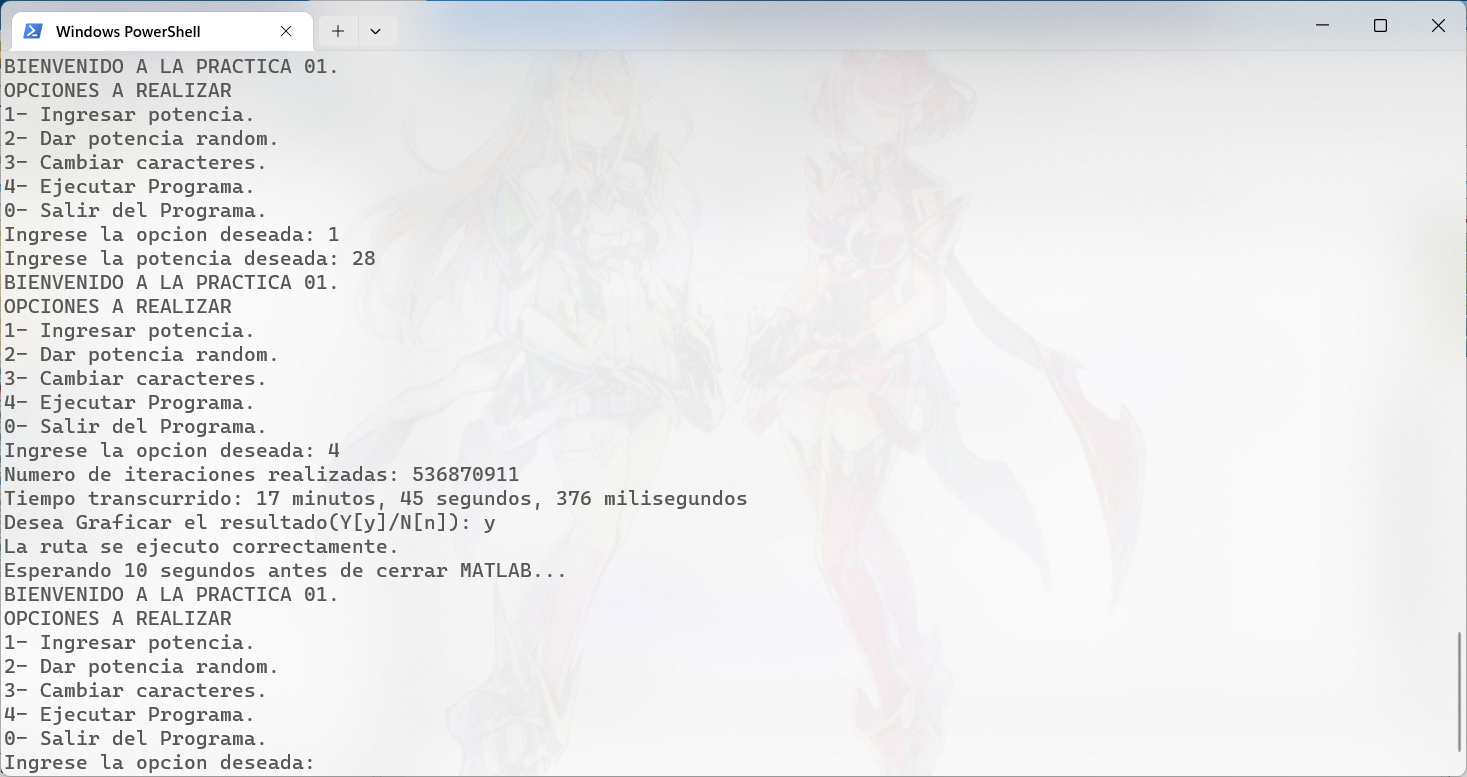
\includegraphics[width=1\linewidth]{Terminal.png}
    \caption{Ejecucion de la Practica 01 en terminal.}\label{terminal}
\end{figure}

\begin{figure}[H]
    \centering
    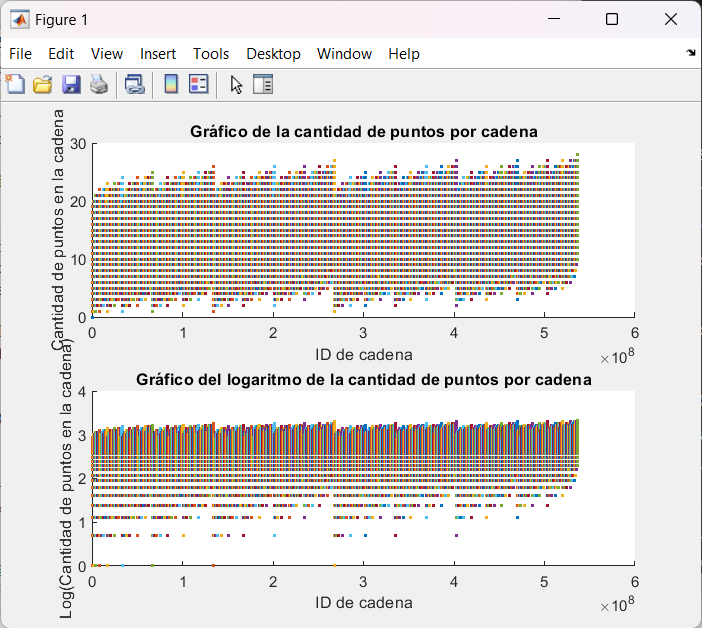
\includegraphics[width=1\linewidth]{Grafico Doble.png}
    \caption{Grafico resultante con potencia = 28}\label{graficaDoble}
\end{figure}

Este es el resultado en el \textit{universo.txt} con una potencia igual a cinco:
\begin{lstlisting}[language={},basicstyle=\ttfamily\footnotesize, breaklines=true]
    e,#,##,###,####,#####,####.,###.,###.#,###..,##.,##.#,##.##,##.#.,##..,
    ##..#,##...,#.,#.#,#.##,#.###,#.##.,#.#.,#.#.#,#.#..,
    #..,#..#,#..##,#..#.,#...,#...#,#....,.,.#,.##,.###,
    .####,.###.,.##.,.##.#,.##..,.#.,.#.#,.#.##,.#.#.,.#..,.#..#,.#...
    ..,..#,..##,..###,..##.,..#.,..#.#,..#..,...,...#,...##,...#.,....,....#,.....
\end{lstlisting}


\section{Conclusiones}
Al completar esta práctica, no solo adquirí conocimientos técnicos en la implementación de algoritmos y la visualización de datos, sino
que experimenté un viaje integral que fusionó la teoría y la práctica en el vasto mundo de la informática. A lo largo de este proceso,
profundicé en los fundamentos de la teoría de autómatas, aplicando conceptos abstractos en la generación de potencias de un alfabeto
utilizando C++. Este ejercicio me permitió no solo entender los principios teóricos detrás de la generación de potencias, sino también
apreciar la importancia de la implementación práctica para comprender plenamente su alcance y aplicación en el mundo real.

Además, al explorar la visualización de datos en MATLAB, descubrí cómo transformar números y conceptos abstractos en imágenes claras y
significativas. La representación gráfica de los datos generados me proporcionó una nueva perspectiva sobre el comportamiento de los
sistemas computacionales, permitiéndome identificar patrones, tendencias y anomalías que de otro modo podrían haber pasado desapercibidos.
Esta experiencia me capacitó para comunicar de manera efectiva los resultados de mis análisis y tomar decisiones informadas basadas en
la evidencia visual.

Más allá de las habilidades técnicas adquiridas, esta práctica me proporcionó una comprensión más profunda de los conceptos
fundamentales que subyacen en el corazón de la computación. Desarrollé una apreciación más amplia de la importancia de la teoría de
autómatas en la construcción y el análisis de sistemas computacionales, así como una comprensión más aguda de cómo la visualización de
datos puede amplificar nuestra capacidad para comprender y tomar decisiones en entornos complejos.

Como conclusion final, puedo decir, esta práctica me equipó con las habilidades y el conocimiento necesarios para abordar desafíos más
complejos en mi viaje en el mundo de la informática y la ciencia de datos. Al integrar teoría y práctica en un viaje de descubrimiento
computacional, avancé hacia un mayor dominio de los principios fundamentales y las herramientas necesarias para enfrentar los desafíos
del futuro con confianza y perspicacia.

\bibliographystyle{ieeetr}
\newpage
\bibliography{referencias}

\end{document}